%%%%%%%%%%%%%%%%%%%%%%%%%%%%%%%%%%%%%%%%%%%%%%%%%%%%%%%%%%%%%%%%%%%%%%

%%% Preamble
\documentclass[	DIV=calc,%
							paper=letter,%
							fontsize=12pt%,%
							%twocolumn
                            ]{scrartcl}	 					% KOMA-article class
\usepackage{float}
\usepackage{lipsum}													% Package to create dummy text

\usepackage[english]{babel}	
\selectlanguage{english}
% English language/hyphenation
\usepackage[protrusion=true,expansion=true]{microtype}				% Better typography
\usepackage{amsmath,amsfonts,amsthm,mathabx}					% Math packages
\usepackage[pdftex]{graphicx}									% Enable pdflatex
\usepackage[svgnames]{xcolor}									% Enabling colors by their 'svgnames'
\usepackage[hang, small,labelfont=bf,up,textfont=it,up]{caption}	% Custom captions under/above floats
\usepackage{epstopdf}												% Converts .eps to .pdf
\usepackage{subfig}													% Subfigures
\usepackage{booktabs}												% Nicer tables
\usepackage{fix-cm}													% Custom fontsizes
\usepackage{cite}
\usepackage{capt-of}
\usepackage[pdftex=false,colorlinks=true,plainpages=true,citecolor=black,linkcolor=black]{hyperref}


%%% Custom sectioning (sectsty package)
\usepackage{sectsty}													% Custom sectioning (see below)
\allsectionsfont{%															% Change font of al section commands
	\usefont{OT1}{phv}{b}{n}%										% bch-b-n: CharterBT-Bold font
	}

\sectionfont{%																% Change font of \section command
	\usefont{OT1}{phv}{b}{n}%										% bch-b-n: CharterBT-Bold font
	}



%%%% Headers and footers
\usepackage{fancyhdr}												% Needed to define custom headers/footers
	\pagestyle{fancy}														% Enabling the custom headers/footers
\usepackage{lastpage}	

% Header (empty)
\lhead{}
\chead{}
\rhead{}
% Footer (you may change this to your own needs)
\lfoot{\footnotesize \texttt{Intelligent Wallet} }
\cfoot{}
\rfoot{\footnotesize Page \thepage\ of \pageref{LastPage}}	% "Page 1 of 2"
\renewcommand{\headrulewidth}{0.0pt}
\renewcommand{\footrulewidth}{0.4pt}
\addto\captionsenglish{\renewcommand{\figurename}{Figure}}
\addto\captionsenglish{\renewcommand{\tablename}{Table}}
\addto\captionsenglish{\renewcommand{\refname}{References}} 


%%% Creating an initial of the very first character of the content
\usepackage{lettrine}
\newcommand{\initial}[1]{%
     \lettrine[lines=3,lhang=0.3,nindent=0em]{
     				\color{DarkGoldenrod}
     				{\textsf{#1}}}{}}



%%% Title, author and date metadata
\usepackage{titling}															% For custom titles

\newcommand{\HorRule}{\color{DarkGoldenrod}%			% Creating a horizontal rule
									  	\rule{\linewidth}{1pt}%
										}

\pretitle{\vspace{-30pt} \begin{flushleft} \HorRule 
				\fontsize{35}{35} \usefont{OT1}{phv}{b}{n} \color{DarkRed} \selectfont 
				}
\title{Intelligent Wallet}					% Title of your article goes here
\posttitle{\par\end{flushleft}\vskip 0.5em}

\preauthor{\begin{flushleft}
					\large \lineskip 0.5em \usefont{OT1}{phv}{b}{sl} \color{DarkRed}}
\author{}											% Author name goes here
\postauthor{\footnotesize \usefont{OT1}{phv}{m}{sl} \color{Black} 
											% Institution of author
					\par\end{flushleft}\HorRule}

\date{}																				% No date

\providecommand{\keywords}[1]
{
  \small	
  \textbf{\textit{Keywords---}} #1
}

%%% Begin document
\begin{document}
\maketitle


\newpage
\begin{abstract}
	
{A chatbot is a technology capable of simulating a human being conversation through a conversational interface. By the use of Artificial Intelligence (AI) and Machine Learning (ML) techniques, it automates the responses to a user through the exchange of messages in what the user perceives as natural language and executes tasks that are designed to transform the experience of the users.

Among diverse types of activities, users might be able to make a reservation   at a restaurant, slide through the product carousels and make a purchase; be notified about canceling a flight to change the ticket at that precise moment and even trace the luggage; it also might be possible to learn how to trade and manage cryptocurrencies through chatbots.

In this paper a design for a cryptocurrency chatbot based on emotions is provided. It answers to queries related to trading and use the human interaction to recognize emotions and predict purchasing intents.}

\end{abstract}

\keywords{chatbot, Artificial Intelligence, Machine Learning, Natural Language Processing, cryptocurrency, emotions}

\newpage
\tableofcontents
\newpage
\listoffigures
\newpage

\thispagestyle{fancy} 			% Enabling the custom headers/footers for the first page 
% The first character should be within \initial{}

\section{\label{sec:level1}Introduction}
Now at days, numerous different web-based services such as e-commerce, e-business, e- learning, etc. are looking for different channels to aid their users. The way companies manage this virtual assistance and their relationship with customers, or as it could be called Customer Relationship Management (CRM), is usually among chat or phone support services. The more increases the demand, more increases the amount of client that must wait for help.  Therefore, a poor client satisfaction is inevitable\cite{ranoliya2017chatbot_08126057}.


One of the aims of Computer Human Interaction(CHI)is to connect with users through instinctive and innate interaction approaches. Natural Language Processing (NLP) has been a wide applied method for this purpose; the user communicates to the computer what is perceived as natural human language and the system is not only able to infer what the user is trying to communicate but also to responds in the same way. \cite{weizenbaum1966eliza_1529899792}\cite{futrelle2009nlp_05332110}.



As result of the need of companies to provide additional services to their customers and the success of NLP, chatbots are positioned as main players of innovation. A chatbot is a technology that makes interaction between man and machine possible by using natural language” and in the past few months, a hype about this topic has been developed\cite{LokmanDesigningDiabetic2009_266872926}. According to Credence Research, chatbots are going to be a key piece of automation for 2019 and they \textit{``are moving aggressively beyond CRM in leading industry verticals. Stand-alone Chatbots are expected to contribute 40\% of the market by 2022''} \cite{Newswire_MarketAssessment2017}.

Chatbots are the result of an evolution of more than 30 years. The first conversational bot was Eliza, invented in the 1960s by the German Joseph Wiezenbaum in the laboratory of Artificial Intelligence from the Massachusetts Institute of Technology (MIT), in U.S. It worked by looking for certain keywords; once a keyword or a tag was detected, ELIZA provided the corresponding response. \cite{ io2017chatbots_08289883}
 
In the 1990s, companies started to implemented telephone IVRs, systems of interactive voice response and in this decade, Richard Wallace developed ALICE. It uses Artificial Intelligence Mark-up Language (AIML) records; they are designed to store information for the chatbot similar an XML.\cite{ wallace2008alice_sn}

Now at day chatbots are getting more popular. An overwhelming increment of 394\% of people tat uses messaging and social apps, as Flurry Analytics reported on 2016, is a factor \cite{khalaf2017their_sn}. Also, thanks to the flexibility of chatbot they have been included in deferments scopes such as e-commerce, e-learning, entertainment, health assistance and every day more applications are being discovered. This without mention the stellar chatbot engines from the big tech companies like IBM Watson, Facebook Messenger, Microsoft XiaoIce, Apple Siri, etc. \cite{ io2017chatbots_08289883}.

\section{\label{sec:level1}Range of Capabilities}
People today want information fast. They have little patience for a subpar experience and they expect answers on their terms and their schedule. This is true across all demographics, but particularly acute amongst younger users.

In many industries now, user experience is perhaps the single most important differentiator, and it is clear that something must change to keep pace with the changing demands of beneficiaries.

Users demand 24/7 attention, immediate, digestible and useful. For the companies this requirement has become an opportunity to improve their customer services models and to add their customer strategies
experience In view of this, chatbots are positioned as main players of innovation. Gartner estimates that more than 85\% of the service centers client, will be operated by bots in 2020.
Brands should become more proactive and anticipate needs of your customers. Managing interactivity will be one of the central functions of the customer experience centers. Intelligent automation will become relevant in the new stage of innovation, driven by the Artificial Intelligence, and a new generation of self-service. 

Omnichannel, real-time attention and simple access to information they have become a challenge to improve the architecture of experiences. The chatbots begin to be understood as one of the ways to improve even completely revolutionize the experience that currently people have with the brands.

A very interesting dumbbell for companies. The metrics that can be obtained help create predictive analytics: what will happen to the market, customers and the business in the near future. Chatbots can become the precise medium for receiving critical information from the business that serves as a basis for new business strategies with a high level of customization and automation.

Chatbots can merge all the services of a company. From the purchase of movie tickets, to booking a hotel or flight, and even answer frequently asked questions and give immediate solution. All through in one messaging application.

Currently the push notifications are the way to do outbound marketing. Brands can schedule promotions and launch them without customization as long day Users are full of notifications out of context.

The chatbots respond to the micromomentos of the people and their level of understanding allows you to make predictions of purchase. For example, if a person bought tickets to watch his favorite team's football game, the chatbot can notify you about the following entries and propose the best seats, suggest that you purchase the special edition cap or you may notice how to get to the stadium, mention nearby parking lots and can even buy food and beverages with a special promotion before reaching the event.

All without having to leave your messaging platform. It will not be necessary that he resorts to the app to buy his tickets or to the web site to consult the prices of souvenirs, or open the browser to trace your route.



\section{\label{sec:level1}Creating User’s Engagement}
Chatbots work most likely humans handle technical support. The chatbot is the medium responding when a customer starts a conversation looking for support. For example, if a trader requests the price of Litecoin, using the information available, the chatbot would immediately respond in the same way as a human would: “George, you recently asked me about Litecoin. Would you like to trade Litecoin, Bitcoin, Ether and 100+ more cryptocurrencies on our new multi-asset trading platform? Click here to find out more”.

A Chatbot can create engagement between business and customers without human interaction. This engagement can be created through small talks: it could be started by sending alerts, for example: “Notify me when a Bitcoin is less than \$7000”; if this event occurs, the chatbot notifies the user adding a call to action “Would you like to trade the Bitcoin now?”. It could broadcast general messages to a wider audience to crate engagement: “Federal Reserve Governor speaks at 3:15pm EST, don’t forget to top up your account!”

Chatbots could also be connected to a trading platform where the chatbot analyze the trader’s exposure to the market and warn of potential threats, for example, “The U.S. Nonfarm Payrolls are out today at 13:30 GMT, which may cause significant volatility. Would you like to manage your positions now?”
 
With the past of the time the chatbot can become smarter by learning from the user’s deposit history, open positions and margin requirements so it can make calls-to-action more targeted: “Your equity is \$1040.34. Should EUR/USD drop more than 100 pips, your position “ Buy 1 lot EUR/USD \@ 1.12345” will be liquidated. Would you like to top up your account to avoid this? The suggested amount is \$450”.

\subsection{\label{sec:level2}User Experience}

The way people communicate is changing in a big way. Just compare the way users communicate today with the way you did 10 or 15 year s ago. If you’re like most people, you have shi f ted away from email and phone calls and toward Facebook Messenger , Whatsapp or even SMS. Like everyone else, you probably prefer communication that is convenient , instantaneous, and always at your fingertips . And, because most of us use our smartphones as our pr imar y PC (not to mention our primary source of contact with other s ) , we prefer communication that i s smartphone- friendly. Messaging apps are the perfect solution. They’re fast and intuitive. The responses you get are short and easy to read. And people like using them.

According to Gartner:
\begin{itemize}
\item 52\% have hung up on a customer service call. 
\item 33\% of Millennials are only willing to wait 1 to 3 minutes to get a response. 
\item 56\% of Millennials have switched from one company to another because of underwhelming customer service.
\end{itemize}


The global use of top messaging applications surpassed the use of the top 4 social networks, and the gap has been growing, as can be evidenced by almost a 400\% increase in the use of Messaging and Social apps in 2016, accordingly to Flurry Analytics.

In just about every country in the world the most frequently used app is a messaging app. They’re pervasive; everyone uses them. And this has been the case for quite some time. Messaging apps surpassed social networks in terms of monthly active users way back in early 2015.
Chatbots can play a role on the frontline of customer service in English —or other languages— to help satisfy the needs of visitors and answer commonly asked questions , to give users what they want, when they need it, as quickly as possible. 

Facebook Messenger is the most commonly used app in North America, while WhatsApp (also owned by Facebook) reigns supreme in Europe and Latin America. In China, WeChat is the hands-down winner. But regardless of the specific app, it is clear that messengers are the channel of choice for people all over the world when communicating with friends \& family.

Messaging apps features the ability to build automated chatbots complete with images, videos, galleries,
call- to-action buttons, and more—making it the app of choice for marketers and business owners looking to grow their business with messenger marketing.

Chatbots can help you to deliver immediate information, and don’t require downloading a separate application - all is done through a familiar messenger window in order to increase user experience. Your chatbot can build a list by attracting new leads, nurture those leads by sending them content and answering their questions, and ultimately convert those leads into new paying customers.

\subsection{\label{sec:level2}Broadcasting and Market Segmentation}

A broadcast is a one-off, manual message that you send to people on your Messenger list. There are three different types of broadcasts you can send on Messenger Marketing, and each type has its own rules and stipulations. As a part of having a positive experience means NOT being inundated with spammy promotional messages.

Subscription Broadcasts: Subscription broadcasts it’s an interactive and individualized experience for the end user. Can not contain promotions or ads, but you can also use subscription broadcasts that ask your subscribers questions. Based off of which button they click, you can then segment them into a sequence where you COULD ultimately sell them something.
Promotional Broadcasts: a broadcast that does contain an ad or other promotional materials. You can only send promotional broadcasts to subscribers who’ve interacted with your brand on in the past 24-hours.
Follow-Up Broadcasts: Follow-up broadcasts give you one last chance to remind your subscribers about your promotion once you send someone a Promotional Broadcast. Brands won’t be able to send any more promotional messages until the subscribers interact with their chatbot again.


Targeting: is where brands can determine who receives the broadcast. Brands can choose to send their broadcast to users who have been tagged in a previous message, users who have subscribed to a specific sequence, or can target by demographics.

Brands can also add multiple conditions to get incredibly focused in the targeting —such as sending a message only to male subscribers who have been tagged as ``likes\_ invest'' and who have not subscribed to your `` Thank You For Invest'' sequence. Eventually you can send them more information about a particular product or promotion based on their needs and interests.
When businesses follow an exponential strategy with their broadcasts, businesses will end up building more of a relationship with the audience. They will come to know and trust businesses, because they did not just ram a single product down their throats— businesses listened to them.




\section{\label{sec:level1}Transactions via Chatbot}

\subsection{\label{sec:level1}Online Trading and Blockchain}

Introducing Intelligent Wallet™ in the transactions sector can bring a huge change in customer experience and keep up the pace with changing customer expectations. Chatbot has the potential to automate all the repetitive questions which are time-consuming and has a huge impact on the departmentís performance. 
The trading industry has a wide range of products and services for its customers. But, not all customers are attentive to every service. Chatbots can deliver personalized offers to customers based on their profile data or life events. Highly-targeted products and services are brought to the customers at the right time by the preferred messaging apps which can intensely increase conversion rates. By using this channel for communication, platforms can achieve a higher market value without annoying the customer.
“There is a lot of interest in the FinTech community in using automated messengers to interact with customers,” Alexey Kulyk, Director of Products at the international payment provider Maxpay, shares, expressing confidence that using messengers and chatbots are more than just a fad. He believes that chatbots are becoming an integral part of any marketing and customer satisfaction plan.
While Apple’s Siri and Amazon’s Alexa are household names now, most chatbots live in social media. There are over 34,000 chatbots on Facebook Messenger alone, providing information to potential customers and driving engagement. Today’s consumers need this extra engagement to be drawn in. Integrating payments capabilities into messaging apps could be the key to making chatbots the next big platform.
A successful chatbot has to be able to perform a task more efficiently than can be done manually. As such, banks should develop chatbots that effectively automate basic and time-consuming tasks. This will free up human staffers' time for more complex inquiries, thus improving customer relations and loyalty.
Currently the push notifications are the way to do outbound marketing.
Brands can schedule promotions and launch them without customization as long day Users are full of notifications out of context.

The chatbots respond to the micromomentos of the people and their level of understanding allows you to make predictions of purchase. For example, if a person bought tickets to watch his favorite team's football game, the chatbot can notify you about the following entries and propose the best seats, suggest that you purchase the special edition cap or you may notice how to get to the stadium, mention nearby parking lots and can even buy food and beverages with a special promotion before reaching the event.

All without having to leave your messaging platform. It will not be necessary that he resorts to the app to buy his tickets or to the web site to consult the prices of souvenirs, or open the browser to trace your route.
 
The basis of blockchain technology is very simple and comes down to the following algorithm: there is a record of transaction operated between two counterparties. It is sent by the DLT to a register journal on regular basis. Each counterparty has their copied sample of register journal. If someone tries to delete or edit details of a transaction, the system will not let them do that because firstly it will compare the record with other counterparties’ register journals.l 

\subsection{\label{sec:level1}Cryptocurrency Services}

Unlike the stock markets, the cryptocurrency market never closes and never sleeps, which can be a highly stressful scenario for traders and even casual investors in the industry. Users familiar with crypto investment will also be familiar with the (joyful or sinking) feeling of waking up in the morning to be greeted by a pleasant or unpleasant surprise when they check their portfolio and see large gains or losses.

The explosion of popularity in cryptocurrency has also resulted in a big increase in the number of trading bots available, either for free from open-source platforms or licensed to users in exchange for flat fees. 

In essence, Intelligent Wallet™ crypto service that interacts directly with financial exchanges (often using API’s to obtain and interpret relevant information) and places buy or sell orders on your behalf depending on the interpretation of the market data. The bots make these decisions by monitoring the market’s price movement and reacting according to a set of predefined and pre-programmed rules. Typically, a trading bot will analyze market actions, such as volume, orders, price, and time, although they can generally be programmed to suit your own tastes and preferences. 


Through the platform two main services can be provided\: Investment Advice and Information Management. The first one has to do with the delivery of recommendations or personalized advices to our users, which suggest the investment decision making about the cryptocurrency. The second one provides Market Information and Individual Account balances.

In order to provide the Investment Advice service Intelligent Wallet ™ requires you to fill some questionnaires  which lead to determine the user's experience with finance, cryptocurrencies,situation and financial capabilities , the investment objective with the finality of give you suitable advices according to their investment needs.




\section{\label{sec:level1}Emotion Detection Engine Potential}

\subsection{\label{sec:level1}Chatbot Engine}
Chatbots have a high level flow where they are in the place where a complete query of the input is made, this is broken down into intentions and identities. An intention is an objective or objective expressed in the entry of a client, such as answering a question or processing an invoice payment. An entity represents an object class or a type of data that is relevant to a user's purpose. By recognizing the entities that are mentioned in the user input, the dialogue system can choose the specific actions that must be performed to fulfill an intention \cite{lee2015natural_sn} \cite{7419068Perzylo_sn}.

For the flow of a dialogue system, first an input is received and processed by intentions detectors to infer in a diffuse way the intentions of the user. In parallel there is also an entity detector which also diffuses, from substrings in the input, the type of entity referred to. Finally a function is called and takes the intentions and the entities as input producing an output, this cycle occurs as many times as necessary. Although there are many variations in the different parts, this structure is the one used in a general way.\cite{lee2015natural_sn}.




\begin{figure}[H]
\centering
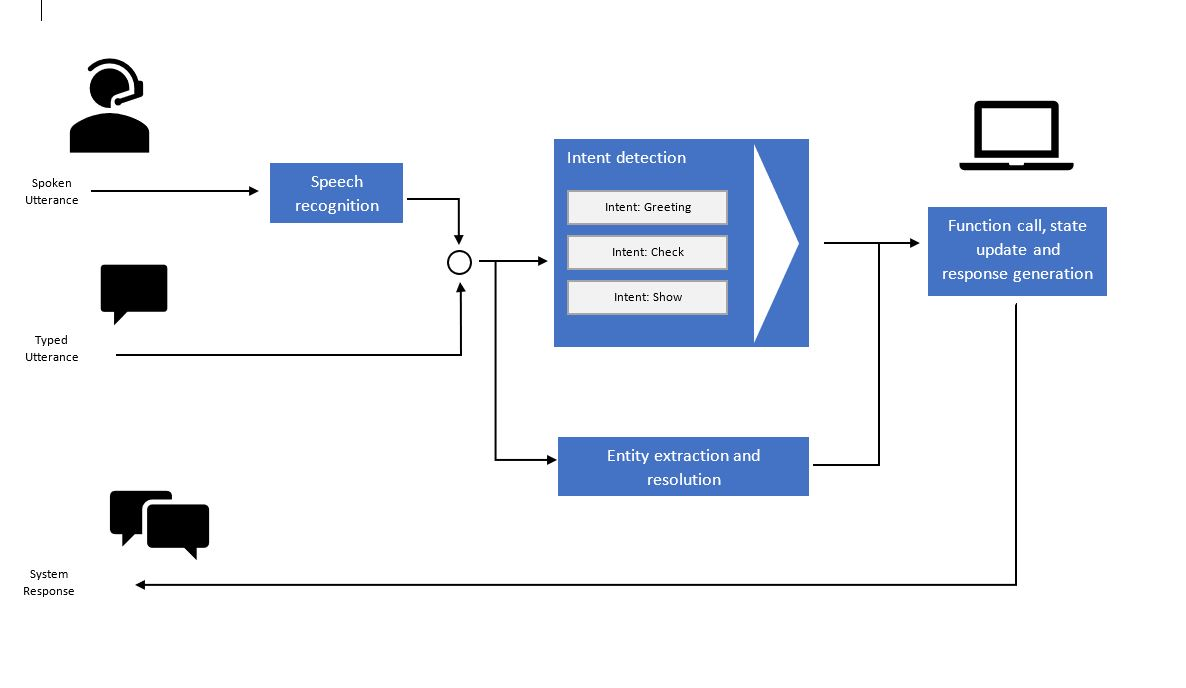
\includegraphics[scale=1.5]{img/Pipeline.JPG}
\caption{Data flow that most dialogue systems possess}
\label{DiagIntent}
\end{figure}


Intelligent Wallet ™ works so that the client specifies one or multiple “Intents” that correspond to a single action or a question the user wants to do. A show.coins intent could, for example, display the best coin to trade during the day for the user. Examples, like “What’s the bullish?” or “Give me the bullish.” The platform can then use these examples with machine learning to match users queries to the correct intent.

Instead of browsing a website, you will have a conversation with the bot, mirroring the type of experience you would get when you go into the complete platform.


%\section{\label{sec:level1}Conclusion}
%Sophisticated chatbots break new ground in conversion and activation of prospects into sales. Being a diligent conversational partner, this AI remembers the history of the dialog and is continuously self-learning. Thus, a chatbot can connect with a user on a more intimate level, it has the ability to get under a traders’ skin by adding value that improves their day-to-day lives. However, only a chatbot with a well-designed architecture and advanced functionality can enrich a company’s communications. \cite{Barbara_CL2018}
%
%Chatbots still remain an underrated channel these days among brokerages, it is an appropriate time to explore whether your business may need one.


\newpage
\bibliography{References}
\bibliographystyle{IEEEtran}
\end{document}